\chapter{Methodology}
\label{chap:methodology}

\section{Framework Architecture Overview}
The proposed framework implements an end-to-end pipeline for generating AI models tailored to motion tracking on edge devices. The system architecture consists of five primary components: (1) data upload and management, (2) interactive preprocessing with visual segmentation, (3) feature extraction, (4) model training with hyperparameter optimization, and (5) platform-specific code generation. The framework is implemented using Python with a Dash web interface, scikit-learn for machine learning, and custom code generators for embedded C++ deployment. Figure \ref{fig:architecture} illustrates the overall workflow.

\begin{figure}[h]
    \centering
    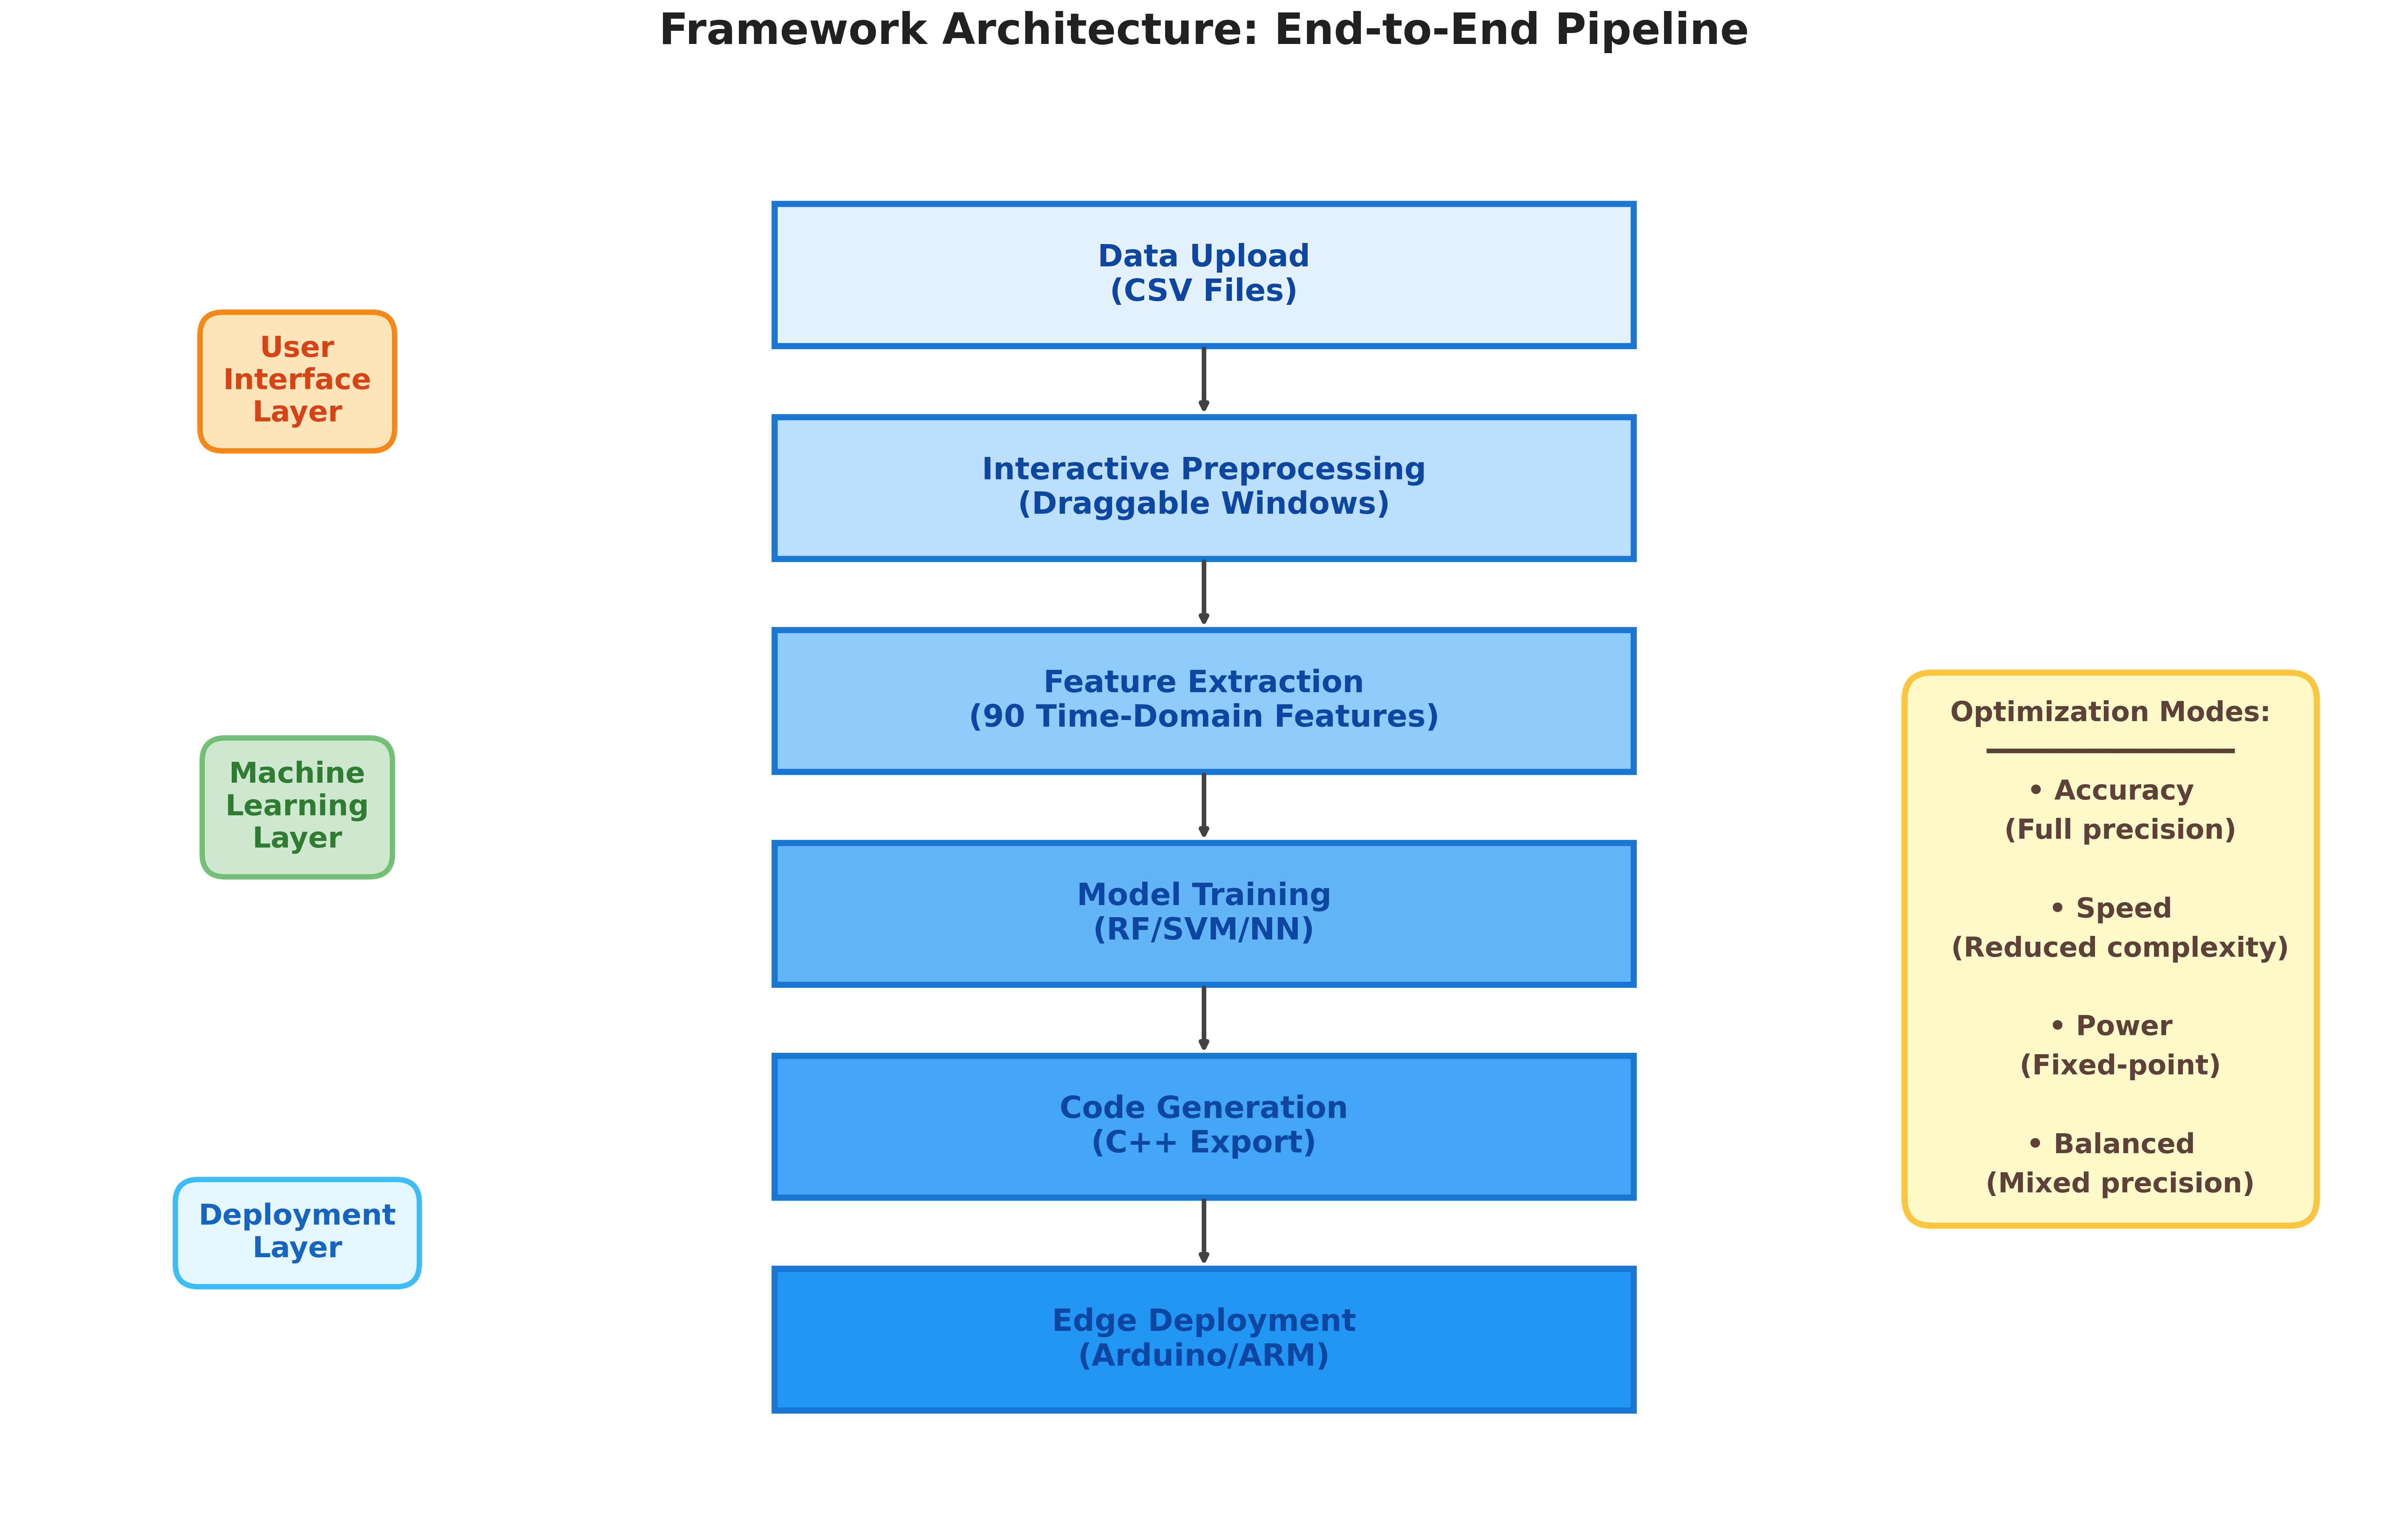
\includegraphics[width=0.85\textwidth]{figures/system_architecture.png}
    \caption{Framework Architecture Overview: End-to-end pipeline from data upload to edge deployment}
    \label{fig:architecture}
\end{figure}

\section{Data Collection and Hardware Platform}

\subsection{Sensor Hardware}
Data collection utilizes the Seeed XIAO nRF52840 Sense microcontroller \cite{web:XIAO}, featuring an ARM Cortex-M4F processor (64MHz, 256KB RAM, 1MB Flash) and an integrated LSM6DS3 6-axis IMU sensor communicating via I2C at address 0x6A. The LSM6DS3 provides 3-axis accelerometer data (configured at $\pm$2g range) and 3-axis gyroscope data, sampled at 100Hz to ensure sufficient temporal resolution for capturing human motion dynamics while balancing memory constraints.

\subsection{Data Acquisition Protocol}
The data collection firmware implements the following procedure:
\begin{enumerate}
    \item Initialize I2C communication and verify IMU connection
    \item Configure accelerometer ($\pm$2g range) and gyroscope sensors
    \item Acquire raw sensor readings at 100Hz (10ms intervals)
    \item Convert accelerometer values to m/s² using conversion factor 9.80665
    \item Maintain gyroscope readings in degrees/second (deg/s)
    \item Output CSV format: aX, aY, aZ, gX, gY, gZ, Time\_seconds
\end{enumerate}

The standardized 100Hz sampling rate ensures consistency between training data collection and real-time inference deployment, eliminating frequency mismatch issues that could degrade model performance.

\section{Interactive Preprocessing Pipeline}

\subsection{Data Upload and Visualization}
Users upload multi-class CSV datasets containing timestamped IMU measurements. The system supports per-activity file organization (e.g., \texttt{walking.csv}, \texttt{running.csv}) where each file corresponds to one activity class. Upon upload, the framework displays synchronized plots of raw accelerometer and gyroscope signals across all six axes, enabling visual inspection of data quality. Figure \ref{fig:ui_data_upload} shows the data upload interface with file selection and initial dataset visualization.

\begin{figure}[H]
    \centering
    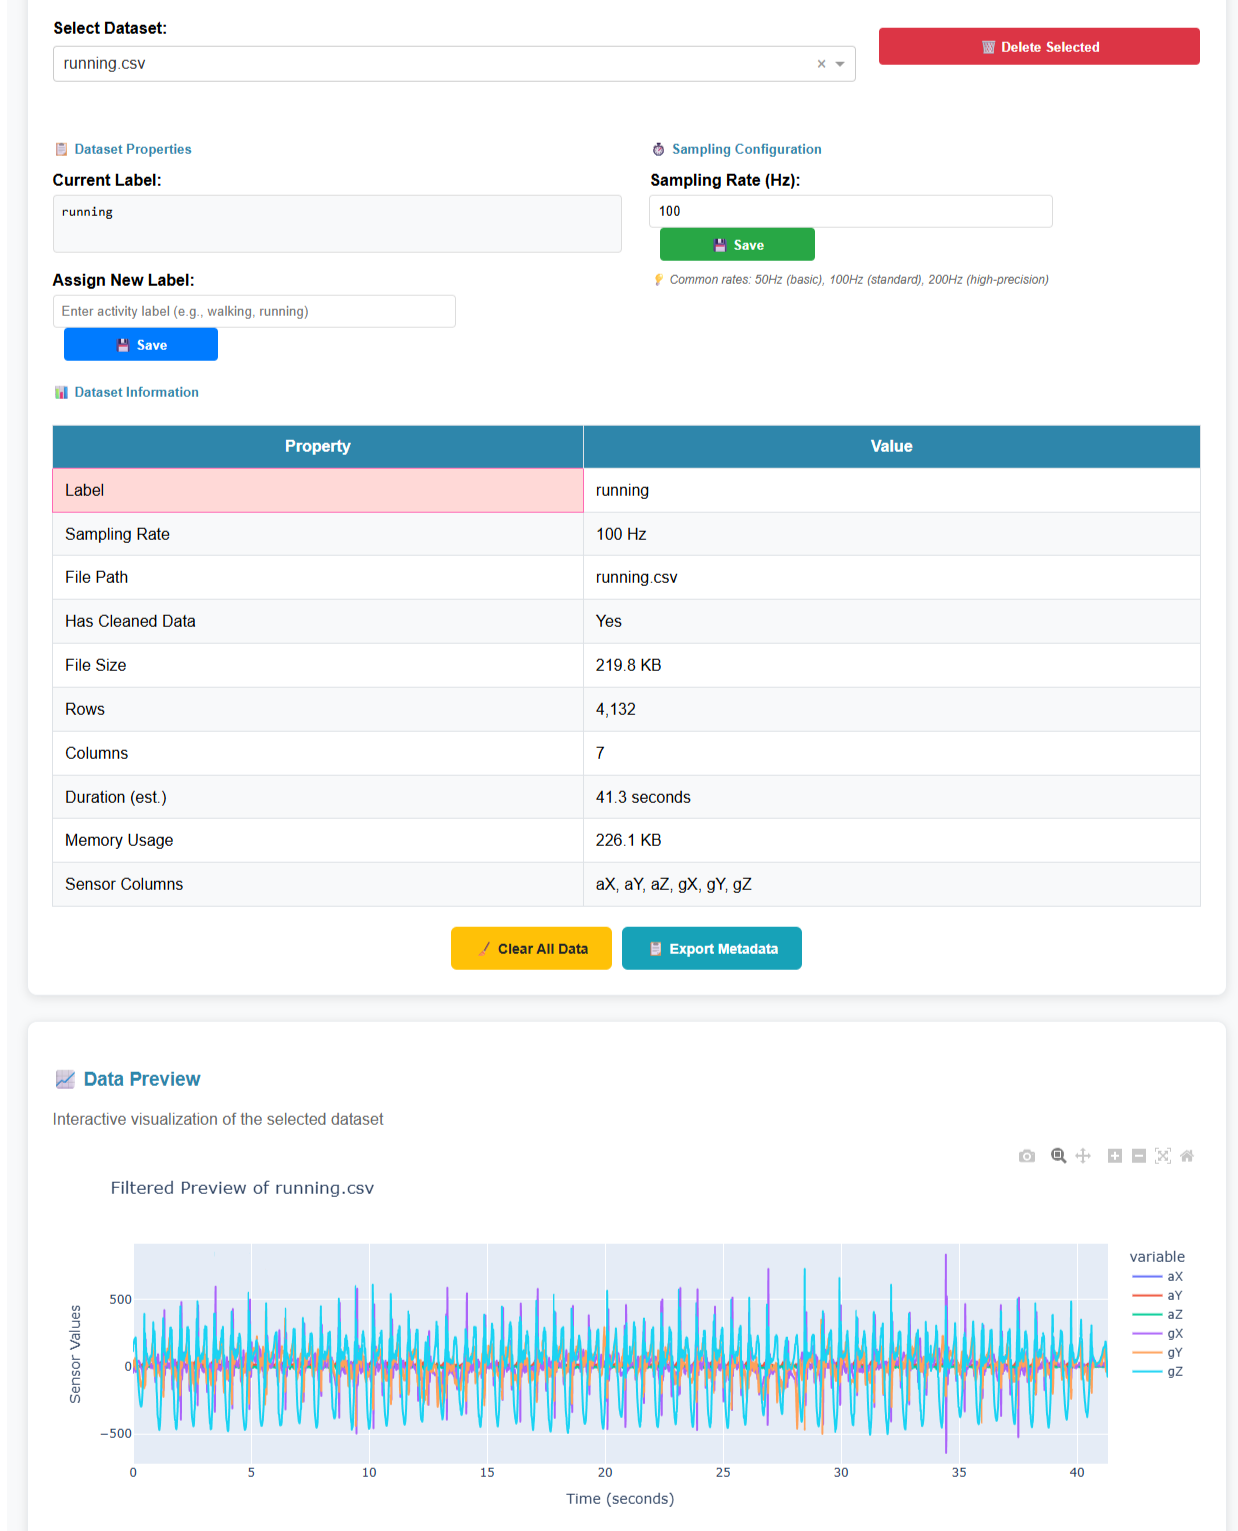
\includegraphics[width=0.95\textwidth]{figures/ui_data_upload.png}
    \caption{Web interface for CSV file upload and dataset management. The interface allows users to upload sensor data files, validates column names, automatically detects sampling frequency, and provides an interactive preview of the raw six-axis time series.}
    \label{fig:ui_data_upload}
\end{figure}

\subsection{Signal Cleaning and Smoothing}
The preprocessing module offers configurable cleaning operations:
\begin{itemize}
    \item \textbf{Outlier Removal}: Identifies and removes samples exceeding specified standard deviation thresholds (default: $3\sigma$), addressing sensor anomalies and electromagnetic interference artifacts.
    \item \textbf{Smoothing}: Applies moving average filters with user-defined window sizes (default: 5 samples) to reduce high-frequency noise while preserving motion characteristics.
\end{itemize}
Cleaned data is visualized alongside original signals, allowing users to verify preprocessing effectiveness before segmentation.

\subsection{Draggable Time Window Segmentation}
A novel contribution of this framework is the \textit{interactive draggable window interface} for activity segmentation. Key features include:
\begin{itemize}
    \item \textbf{Visual Window Placement}: Users click-and-drag directly on signal plots to define temporal boundaries of activity instances, providing intuitive control over segmentation without coding.
    \item \textbf{Multi-Window Support}: Multiple non-overlapping windows can be defined per activity file, accommodating datasets with multiple instances of the same activity.
    \item \textbf{Real-Time Feedback}: Selected windows are highlighted on the plot with distinct colors, and extracted segments are immediately available for inspection.
    \item \textbf{Per-Window Labeling}: Each window is automatically assigned the activity label from the parent file, but can be manually re-labeled if needed (e.g., extracting \textit{standing} segments from \textit{walking} files during transition periods).
\end{itemize}
This approach significantly reduces annotation time compared to manual timestamp entry or programmatic segmentation, and eliminates common errors in boundary specification. Figure \ref{fig:ui_preprocessing} demonstrates the interactive draggable window interface, which is the key differentiating feature of this framework.

\begin{figure}[H]
    \centering
    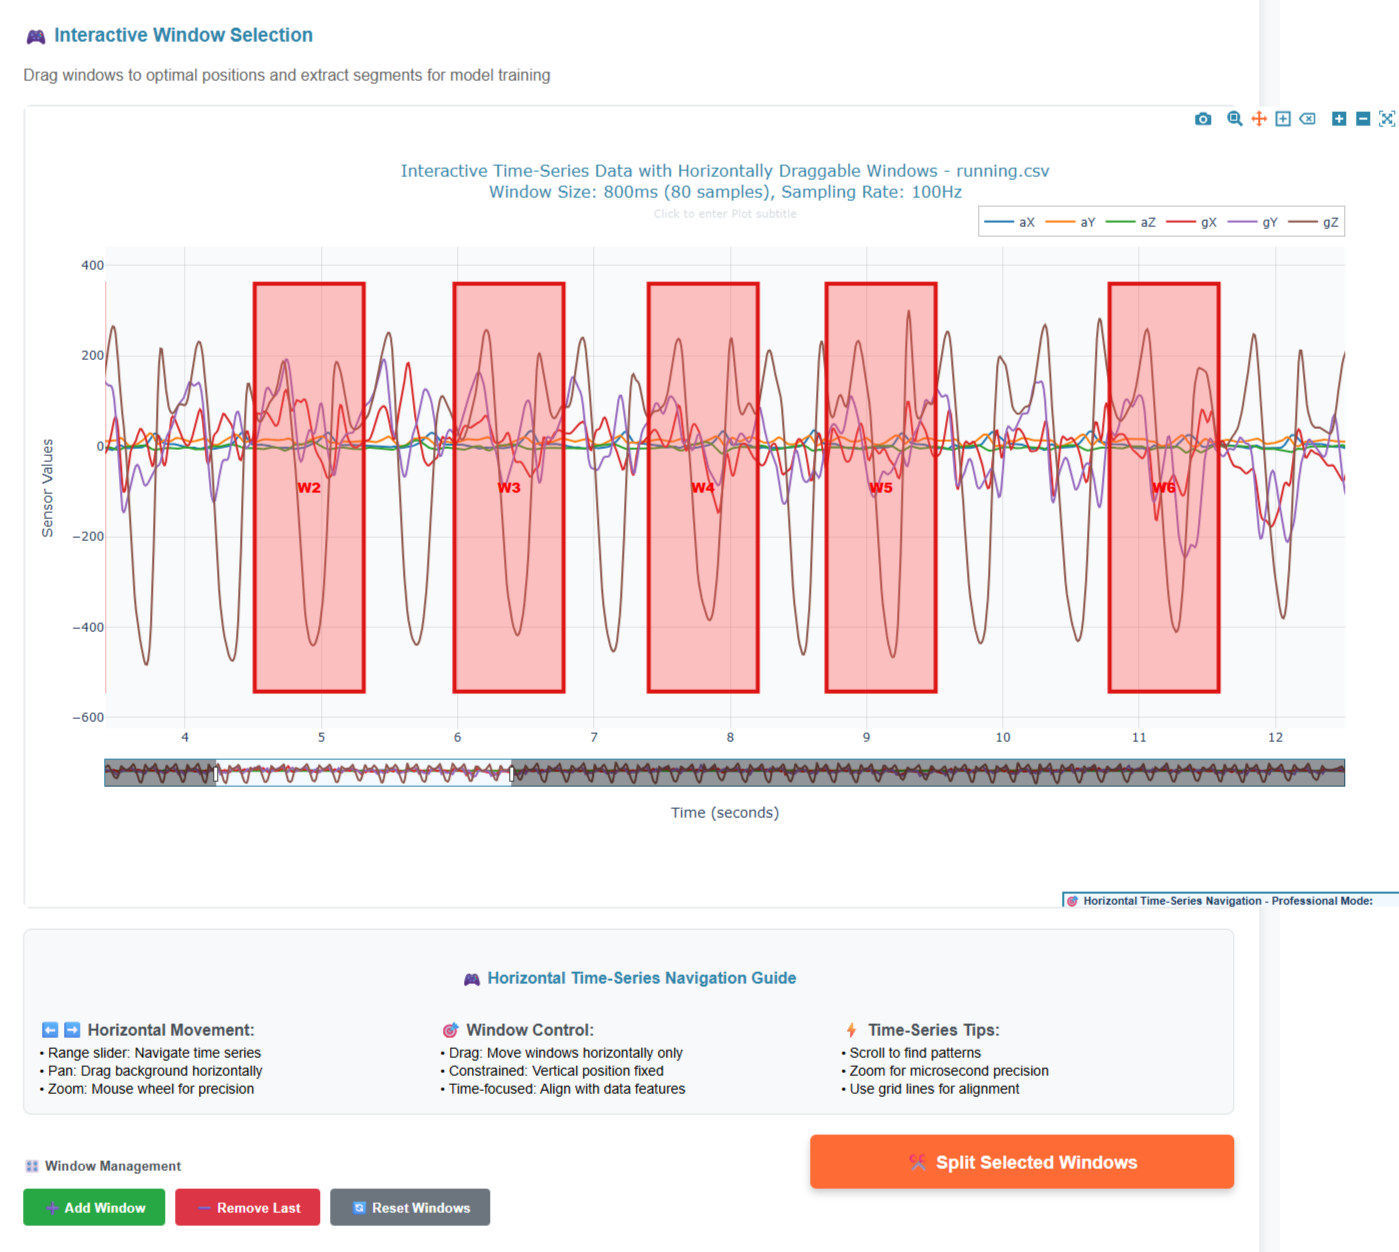
\includegraphics[width=0.95\textwidth]{figures/ui_preprocessing_draggable.png}
    \caption{Interactive draggable window interface for activity segmentation. Users visually inspect accelerometer and gyroscope time series, drag rectangular windows over regions corresponding to distinct activities, assign activity labels, and adjust boundaries via click-and-drag interaction. This eliminates manual timestamp calculation and makes the framework accessible to non-programmers.}
    \label{fig:ui_preprocessing}
\end{figure}

\section{Feature Extraction}
\label{sec:feature_extraction}

\subsection{Sliding Window Approach}
Preprocessed signals are segmented into fixed-size overlapping windows for feature extraction. After empirical validation and comparison with literature recommendations \cite{banos2014wisdm}, the configuration was optimized as:
\begin{itemize}
    \item \textbf{Sampling Rate}: 100Hz (fixed)
    \item \textbf{Window Size}: 150 samples (1.5 seconds at 100Hz)
    \item \textbf{Overlap}: 50\% (75-sample stride)
\end{itemize}
The 1.5-second window provides sufficient temporal context to capture complete motion cycles for most activities (walking step duration $\approx$ 1.0-1.2 seconds \cite{whittle2014gait}), while 50\% overlap ensures temporal continuity and reduces edge effects at window boundaries. This yields predictions every 0.75 seconds, balancing responsiveness with computational efficiency.

\textit{Implementation Note}: These parameters are currently hardcoded in both the training pipeline (\texttt{utils/model\_training.py}) and code generation module (\texttt{deployment/base\_generator.py}) to ensure training-deployment consistency. Future work could expose these as user-configurable parameters with validation to prevent incompatible configurations. The framework assumes labeled samples exceed the minimum window size (1.5 seconds); shorter segments are not zero-padded and may produce invalid features.

\subsection{Feature Set}
For each window and each sensor axis (6 axes total), the framework extracts 15 time-domain statistical features. Frequency-domain features were intentionally excluded after identifying training-deployment parity issues: FFT implementations differ substantially between Python (NumPy) and embedded C++ (approximations or ARM CMSIS-DSP), leading to feature value discrepancies that degrade deployed model accuracy.

\textbf{Rationale for Excluding FFT Features}: While frequency-domain features (spectral energy, dominant frequency, spectral entropy) are commonly used in HAR literature \cite{banos2014wisdm}, they introduce significant deployment challenges. Python's NumPy FFT uses highly optimized double-precision floating-point algorithms (FFTPACK/FFTW backends), while embedded C++ typically relies on fixed-point approximations or platform-specific libraries (ARM CMSIS-DSP) with different numerical precision. Preliminary experiments revealed that identical input windows produced FFT magnitude spectra differing by 5-15\% between Python and C++, causing trained models to misclassify 8-12\% of windows during deployment despite 95\%+ training accuracy. This "training-deployment mismatch" is a critical but under-reported issue in edge ML \cite{banbury2021mlperf}. By restricting to time-domain features with deterministic closed-form computations (mean, variance, etc.), we guarantee bit-identical feature extraction across platforms, eliminating this failure mode. The zero-crossing rate and mean-crossing rate serve as frequency proxies, capturing periodic information without FFT overhead.

\textbf{Time-Domain Features (15 per axis):}
\begin{itemize}
    \item \textbf{Central Tendency}: Mean, Median
    \item \textbf{Dispersion}: Standard Deviation, Variance, Range (Max - Min), Interquartile Range (IQR)
    \item \textbf{Extrema}: Minimum, Maximum, 25th Percentile (Q1), 75th Percentile (Q3)
    \item \textbf{Shape}: Skewness $\gamma = \frac{E[(X-\mu)^3]}{\sigma^3}$, Kurtosis $\kappa = \frac{E[(X-\mu)^4]}{\sigma^4} - 3$ (bias-corrected)
    \item \textbf{Energy}: Root Mean Square (RMS) $= \sqrt{\frac{1}{N}\sum_{i=1}^{N} x_i^2}$, Signal Energy $E = \sum_{i=1}^{N} x_i^2$
    \item \textbf{Frequency Proxy}: Zero-Crossing Rate, Mean-Crossing Rate (signal crossings over mean)
\end{itemize}

Total feature vector dimensionality: $15 \times 6 = 90$ features per window. This time-domain-only approach ensures perfect parity between training (Python pandas/NumPy) and deployment (C++ direct computation), critical for achieving consistent model performance on edge devices. The comprehensive statistical representation captures motion amplitude, dynamics, distribution characteristics, and pseudo-frequency information sufficient for discriminating activities with distinct biomechanical signatures.

\section{Machine Learning Model Training}

\subsection{Supported Algorithms}
The framework integrates three classical machine learning algorithms from scikit-learn, selected for their proven effectiveness in activity recognition and feasibility for embedded deployment:

\paragraph{Random Forest (RF)}
Ensemble method combining multiple decision trees with bagging and feature randomization. Configuration:
\begin{itemize}
    \item Default: 100 trees, max depth 20
    \item Class balancing: \texttt{class\_weight='balanced'} automatically weights samples inversely proportional to class frequency
    \item Criterion: Gini impurity
\end{itemize}

\paragraph{Support Vector Machine (SVM)}
Discriminative classifier finding optimal hyperplanes via kernel methods. Configuration:
\begin{itemize}
    \item Kernel: Radial Basis Function (RBF) with automatic gamma scaling
    \item Multi-class strategy: One-vs-One (OvO)
    \item Class balancing: \texttt{class\_weight='balanced'}
    \item Regularization: C=1.0 (default)
\end{itemize}

\paragraph{Neural Network (NN)}
Multi-layer perceptron with backpropagation. Configuration:
\begin{itemize}
    \item Architecture: 90 input $\rightarrow$ 100 hidden $\rightarrow$ 50 hidden $\rightarrow$ num\_classes output
    \item Activation: ReLU (hidden layers), Softmax (output layer)
    \item Optimizer: Adam with learning rate 0.001, $\beta_1=0.9$, $\beta_2=0.999$
    \item Regularization: L2 penalty $\alpha=0.0001$
    \item Training: Early stopping with patience=10, max 500 epochs
    \item Batch size: Full batch (entire training set)
\end{itemize}
The two-hidden-layer architecture provides sufficient capacity for learning non-linear activity patterns while remaining small enough for efficient C++ deployment (fixed-weight matrices, no dynamic memory allocation).

\subsection{Training and Evaluation Protocol}

\subsubsection{Data Splitting Strategy}
The framework implements a rigorous three-way split to prevent information leakage and ensure unbiased performance estimates:
\begin{enumerate}
    \item \textbf{Training Set (60\%)}: Used exclusively for model training (fitting model parameters)
    \item \textbf{Validation Set (20\%)}: Used for hyperparameter tuning, model selection, and monitoring training progress
    \item \textbf{Test Set (20\%)}: Completely held-out for final evaluation only; never accessed during training or hyperparameter optimization
\end{enumerate}

All splits use stratified sampling to preserve class proportions across sets, critical for imbalanced activity recognition tasks.

\textit{Validation vs. Test Set Distinction}: The validation set enables iterative model development—users can tune hyperparameters, try different algorithms, or adjust preprocessing steps while monitoring validation accuracy without contaminating the test set. The test set is evaluated \textit{exactly once} per trained model to report final performance, providing an unbiased estimate of generalization to unseen data. This methodology follows best practices in machine learning research \cite{goodfellow2016deep} and eliminates the subtle information leakage that occurs when repeatedly evaluating on a single held-out set.

\textit{Cross-Validation Option}: For exploratory analysis, the framework also supports 5-fold cross-validation performed on the combined training+validation set (80\% of data), while still preserving the test set (20\%) as completely unseen. This provides robust performance estimates for algorithm comparison studies without requiring a separate validation split.

\subsubsection{Class Imbalance Handling}
Motion datasets often exhibit severe class imbalance (e.g., more \textit{standing} samples than \textit{walking\_downstairs}). Imbalanced training biases models toward majority classes, degrading minority class recognition. The framework addresses this via:
\begin{itemize}
    \item \textbf{Class Weight Balancing}: For RF and SVM, the \texttt{class\_weight='balanced'} parameter assigns weights $w_c = \frac{n\_samples}{n\_classes \times n\_samples_c}$ where $n\_samples_c$ is the count of class $c$. This increases the loss contribution of minority class misclassifications during training.
    \item \textbf{Stratified Splitting}: Train-test splits preserve class proportions using stratified sampling.
\end{itemize}
Class balancing is crucial for real-world deployment where all activity classes must be reliably detected, not just the most frequent ones.

\subsection{Hyperparameter Optimization}
The framework supports automated hyperparameter tuning via scikit-learn's GridSearchCV with 5-fold cross-validation. Searchable hyperparameters:

\textbf{Random Forest:}
\begin{itemize}
    \item \texttt{n\_estimators}: [50, 100, 200]
    \item \texttt{max\_depth}: [10, 20, 30, None]
    \item \texttt{min\_samples\_split}: [2, 5, 10]
    \item \texttt{class\_weight}: ['balanced', 'balanced\_subsample']
\end{itemize}

\textbf{SVM:}
\begin{itemize}
    \item \texttt{C}: [0.1, 1, 10, 100]
    \item \texttt{gamma}: ['scale', 'auto', 0.001, 0.01, 0.1]
    \item \texttt{class\_weight}: ['balanced']
\end{itemize}

\textbf{Neural Network:}
\begin{itemize}
    \item \texttt{hidden\_layer\_sizes}: [(50,), (100,), (100, 50)]
    \item \texttt{alpha}: [0.0001, 0.001, 0.01]
    \item \texttt{learning\_rate\_init}: [0.001, 0.01]
\end{itemize}

Optimization identifies configurations maximizing cross-validation accuracy, typically improving baseline performance by 2-5\%. Figure \ref{fig:ui_training} shows the training configuration interface where users select algorithms, enable hyperparameter optimization, configure class balancing, and monitor training progress.

\begin{figure}[H]
    \centering
    
\includegraphics[width=0.95\textwidth]{figures/ui_training_config.png}
    \caption{Model configuration panel showing algorithm selection (Random Forest, Neural Network, SVM), hyperparameter tuning options with GridSearchCV, class balancing strategies (balanced weights, stratified splitting), and real-time training progress monitoring with cross-validation scores.}
    \label{fig:ui_training}
\end{figure}

\section{Code Generation for Edge Deployment}

\subsection{Architecture}
The code generation subsystem translates trained scikit-learn models into standalone C++ implementations executable on microcontrollers without external dependencies. Architecture follows the Factory design pattern with inheritance:
\begin{itemize}
    \item \textbf{BaseCodeGenerator}: Abstract class with common functionality\\(file structure, serialization, validation).
    \item \textbf{Model-Specific Generators}: Subclasses implementing algorithm-specific prediction logic:
    \begin{itemize}
        \item \texttt{SVMGenerator}: RBF kernel computation, support vector storage, multi-class decision scoring
        \item \texttt{NeuralNetworkGenerator}: Forward propagation through hidden/output layers, activation functions (ReLU, sigmoid)
\item \texttt{RandomForestGenerator}: Binary tree traversal, majority voting.
        \item \texttt{ARMCortexGenerator}: Fixed-point arithmetic, ARM CMSIS-DSP optimizations (optional)
    \end{itemize}
\end{itemize}

\subsection{Generated Code Structure}
For each trained model, the generator produces three files:
\begin{enumerate}
    \item \textbf{Header File (.h)}: Contains model parameters (e.g., support vectors, tree structures, weight matrices), function declarations, feature count/class count macros
    \item \textbf{Implementation File (.cpp)}: Implements feature extraction, prediction logic (algorithm-specific), and utility functions
    \item \textbf{Arduino Sketch (.ino)}: Provides sensor initialization, sliding window buffer management, real-time inference loop, and serial output of predictions
\end{enumerate}

Figure \ref{fig:ui_code_generation} shows the code generation interface with a preview of the generated Arduino C++ code, deployment configuration options, and downloadable output files.

\begin{figure}[H]
    \centering
    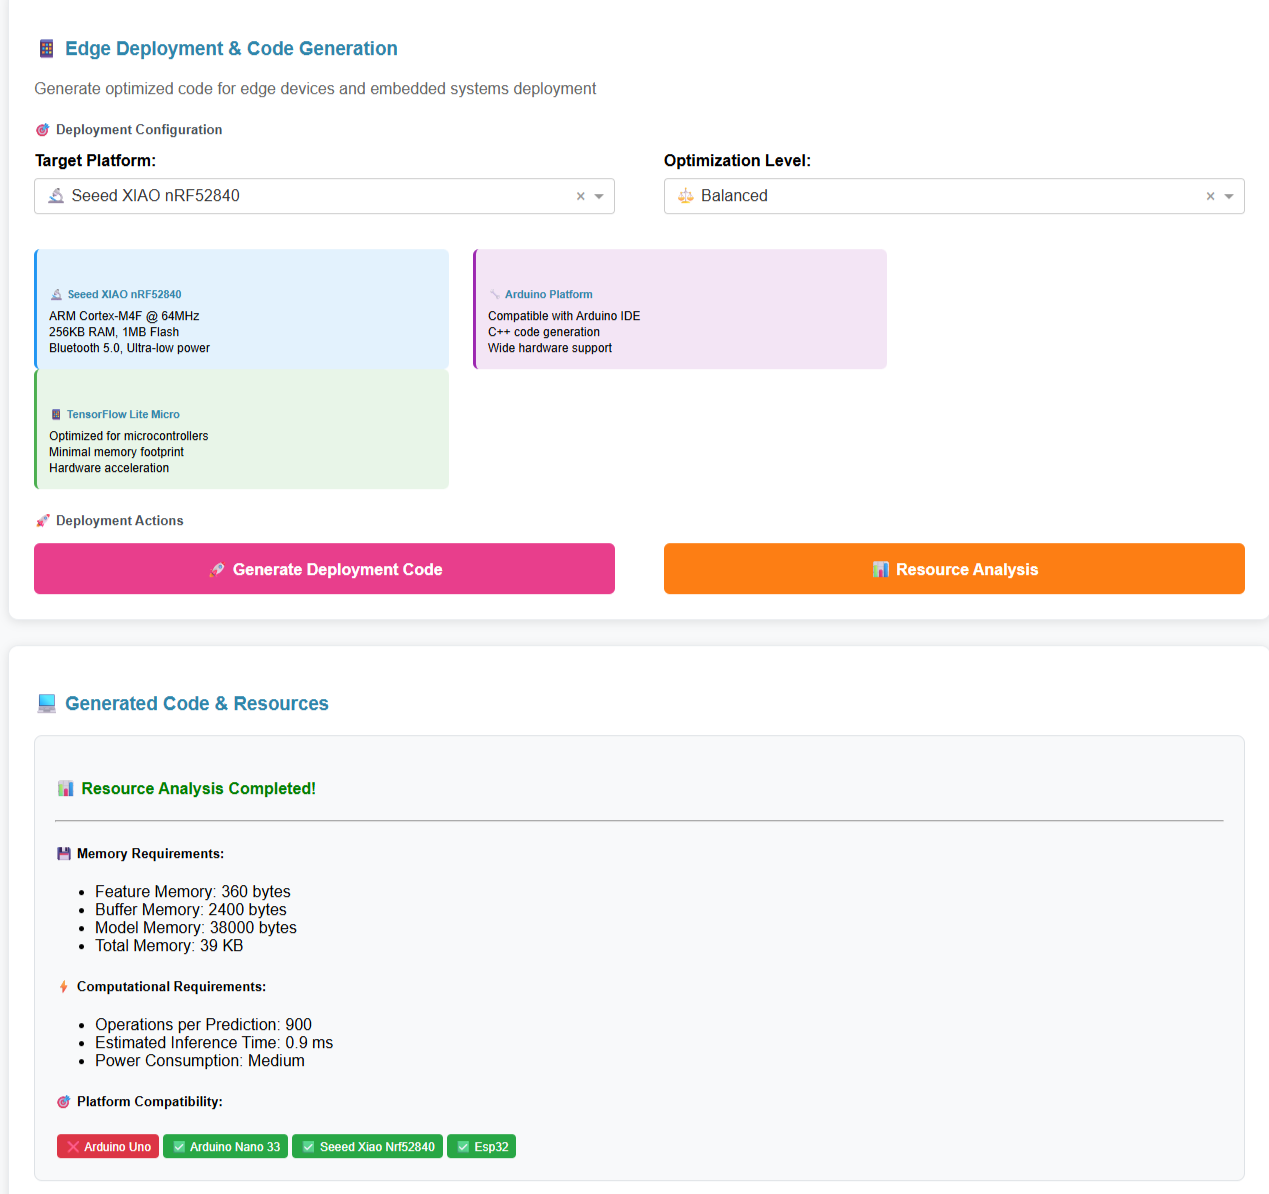
\includegraphics[width=0.95\textwidth]{figures/ui_code_generation.png}
    \caption{Generated Arduino C++ code preview interface. The framework displays the generated header files, implementation files, and Arduino sketches with syntax highlighting. Users can select optimization modes (Accuracy, Speed, Power, Balanced), configure target platform parameters, and download the complete deployment package.}
    \label{fig:ui_code_generation}
\end{figure}

\subsection{Optimization Strategies}
The framework supports four deployment optimization modes, selectable during code generation:

\paragraph{Accuracy Mode}
Prioritizes prediction correctness:
\begin{itemize}
    \item Full-precision floating-point arithmetic
    \item No model simplification (all trees/support vectors retained)
    \item Complete feature set (90 time-domain features)
\end{itemize}

\paragraph{Speed Mode}
Minimizes inference latency:
\begin{itemize}
    \item Reduced model complexity (fewer trees, reduced SVM support vectors via pruning)
    \item Optimized feature computation order (cache-friendly access patterns)
    \item Loop unrolling and inlined functions
\end{itemize}

\paragraph{Power Mode}
Reduces energy consumption:
\begin{itemize}
    \item Fixed-point integer arithmetic where feasible
    \item Reduced sampling frequency (configurable down to 50Hz)
    \item Sleep modes between inference cycles (not implemented in current version)
\end{itemize}

\paragraph{Balanced Mode}
Compromises between accuracy, speed, and power:
\begin{itemize}
    \item Moderate model complexity
    \item Selective feature set (top 60-75 features by importance)
    \item Mixed precision (critical computations in float, intermediate in fixed-point)
\end{itemize}

\subsection{Platform-Specific Adaptations}
While the framework currently targets Arduino-compatible platforms (Seeed XIAO, ESP32, Arduino Nano 33 BLE), the modular architecture supports platform-specific adaptations:
\begin{itemize}
    \item \textbf{Memory Layout}: Adjusts array storage (PROGMEM for AVR, const for ARM) based on flash/RAM availability
    \item \textbf{Hardware Acceleration}: ARM Cortex-M platforms can leverage CMSIS-DSP library for SIMD operations on feature computation
    \item \textbf{Sensor Drivers}: Abstracts sensor initialization to support different IMU models (LSM6DS3, MPU6050, BNO055)
\end{itemize}

\section{Experimental Design}

\subsection{Dataset}
Validation experiments use a Human Activity Recognition (HAR) dataset collected from a single subject performing five activities:
\begin{itemize}
    \item \textit{Running}, \textit{Still}, \textit{Walking}, \textit{Walking Downstairs}, \textit{Walking Upstairs}
\end{itemize}
Data was collected using the Seeed XIAO nRF52840 Sense platform at 100Hz over multiple recording sessions. Each activity was recorded for 30-60 seconds across multiple sessions, with careful attention to transitional periods. The draggable window interface was used to segment continuous recordings into \textbf{labeled samples} (manually-annotated activity segments), extracting multiple representative windows per activity. 

\textit{Feature Extraction Process}: Each labeled sample (typically 30-60 seconds long) is then processed using the sliding window approach (Section~\ref{sec:feature_extraction}) with 1.5-second windows and 50\% overlap. This transforms the labeled samples into 159 \textbf{feature vectors} (training data points) that are split into training (101 samples, 63.5\%), validation (28 samples, 17.6\%), and test sets (30 samples, 18.9\%). The dataset contains five activity classes:
\begin{itemize}
    \item Running: 30 total samples (18.9\%)
    \item Still: 30 total samples (18.9\%)
    \item Walking: 30 total samples (18.9\%)
    \item Walking Downstairs: 35 total samples (22.0\%)
    \item Walking Upstairs: 34 total samples (21.4\%)
\end{itemize}
Class imbalance ratio: 1.17:1 (walking downstairs vs. running/still/walking), representing a relatively balanced dataset suitable for demonstrating class weight effectiveness without extreme imbalance. Each feature vector contains 90 time-domain features (15 features × 6 sensor axes).

\subsection{Evaluation Metrics}
Model performance is assessed using:
\begin{itemize}
    \item \textbf{Overall Accuracy}: Percentage of correctly classified windows
    \item \textbf{Per-Class Precision}: $P_c = \frac{TP_c}{TP_c + FP_c}$
    \item \textbf{Per-Class Recall}: $R_c = \frac{TP_c}{TP_c + FN_c}$
    \item \textbf{F1-Score}: Harmonic mean of precision and recall
    \item \textbf{Confusion Matrix}: Visualizes misclassification patterns
\end{itemize}

Edge deployment performance is measured via:
\begin{itemize}
    \item \textbf{Inference Time}: Average time to classify one 150-sample window (ms), measured using Arduino \texttt{micros()} timing over 100 consecutive predictions on the target hardware
    \item \textbf{Memory Usage}: Flash (program storage) and SRAM (runtime variables/buffers) consumption (KB), extracted from compiler map files and Arduino IDE build output showing actual compiled binary sizes
    \item \textbf{Power Consumption}: Average current draw during different operational phases (idle, sensor sampling, feature extraction, prediction). \textit{Note: Power values reported in this thesis are estimates calculated from typical ARM Cortex-M4F current consumption specifications (8-12 mA active, 2-3 mA idle at 64MHz) and measured execution time percentages, not direct hardware measurements with power monitors (e.g., Joulescope, Nordic PPK2). Actual power consumption may vary $\pm$15-20\% based on specific hardware implementation, sensor characteristics, and environmental factors. Future work should validate these estimates with hardware power profiling equipment.}
    \item \textbf{Prediction Frequency}: Sustainable inference rate accounting for sensor sampling overhead (predictions per second)
\end{itemize}
Target performance thresholds based on application requirements: inference $<$ 100ms per window (enabling real-time 10Hz updates), flash $<$ 500KB (leaving headroom for application code), SRAM $<$ 128KB (50\% of available 256KB), power $<$ 50mW average (supporting multi-hour battery operation).

\subsection{Baseline Comparisons}
To contextualize framework performance, we compare against:
\begin{enumerate}
    \item \textbf{Edge Impulse}: Commercial platform with automated pipeline (free tier limitations apply)
    \item \textbf{Manual TensorFlow Lite Deployment}: Represents expert-level custom implementation
    \item \textbf{Unbalanced Training}: Same framework but without class weight balancing (ablation study)
\end{enumerate}

\section{Implementation Details}
\textbf{Software Stack:}
\begin{itemize}
    \item Python 3.10 with Dash 2.14 (web interface)
    \item scikit-learn 1.3 (machine learning)
    \item NumPy, Pandas (data processing)
    \item Plotly (visualization)
\end{itemize}

\textbf{Hardware:}
\begin{itemize}
    \item Development: Windows 11 workstation (Intel i7, 16GB RAM)
    \item Deployment: Seeed XIAO nRF52840 Sense (ARM Cortex-M4F @ 64MHz, 256KB RAM, 1MB Flash)
    \item Sensor: LSM6DS3 6-axis IMU (I2C, 100Hz sampling)
\end{itemize}

\textbf{Code Availability:}
The framework source code, example datasets, and deployment examples are available in the project repository.